\section{Digital Communication Interface and Readout}
\label{sec:logic_design}


\subsection{Description of the ASIC digital subsystem}
\label{sec:descriptionASIC}


\begin{figure}[H]
    \centering
    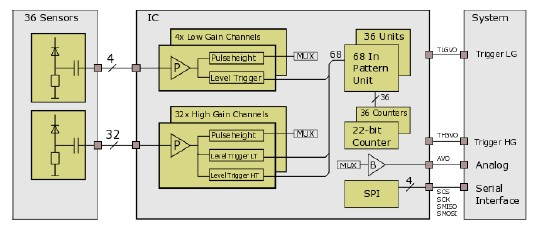
\includegraphics[width=1\textwidth]{ASIC_schematic.jpg}
    \caption[]{Block Diagram Schematic of the ASIC (VATA466/ide3466) (\cite{Meier2016VATA466}) }
    \label{fig:ASIC_schematic}
\end{figure}

\subsubsection{Input Channels}

From the figure above it can be seen that each diode anode is AC-coupled to one input. The ASIC has 4 Low Gain (LG) channels and 32 High Gain (HG) channels, which serve as input from the detector diodes of the directionality sensor. Each channel has one pre-amplifier and an analogue processing for pulse height and level triggers. In the figure below, the channel inputs are depicted on the left side of the scheme.

\begin{figure}[H]
    \centering
    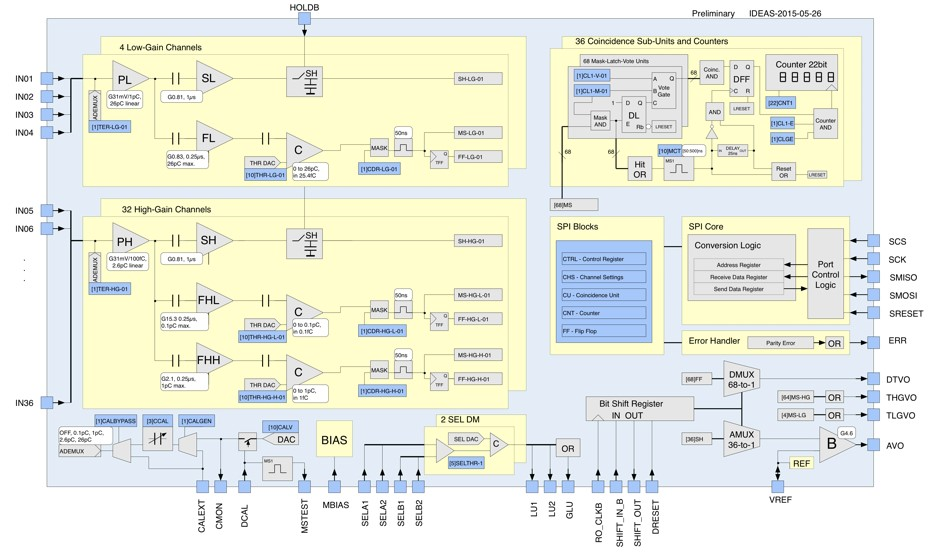
\includegraphics[width=0.9\textwidth]{ASIC_Functional.jpg}
    \caption[]{ASIC functional schematic with I/O (VATA466/ide3466) (\cite{Meier2016VATA466}) }
    \label{fig:ASIC_Functional}
\end{figure}

\subsubsection{Modes of operation}

The ASIC has two modes of operation and each of the modes requires a different approach for the readout. It can be used in the Counting Mode Acquisition (CMA) or Spectroscopic Mode Acquisition (SMA). 
\newline
The CMA is the mode for which the digital hardware was designed. In this mode, the values of a total of 36 registers, which comprise the so-called Coincidence Sub-Unit (CSU) of the ASIC, can be read. The CMU, its registers and configuration principle is described later in this section. The value in each of the registers reflects the number of events that occurred, which fulfill the requirements of any individual out of 36 prior defined coincidences.
\newline
The following steps are required to run this mode successfully:





\begin{itemize}
\item Configuration of the analogue channel thresholds through channel configuration registers

\item Configuration of the coincidence units with channel trigger coincidence and anti-coincidence through Coincidence Sub-Unit configuration registers
\item Periodic read-out of the coincidence counter registers

\end{itemize}

The SMA mode will only be explained briefly in this report.
Its objective is to recreate the shape of the detected
pulses. The pulses which are registered in the input
channels can be transformed to 36 analogue values by a slow
shaper and can be later read out serially with the help of
an analogue multiplexer (36-to-1 AMUX) that is controlled
by the RO\_CLKB, SHIFT\_IN\_B and DRESET inputs as seen in
\ref{fig:ASIC_Functional}, the signal SHIFT\_OUT
indicates when the operation is finished.

The parts of the subsystem will be described with regards to the counting mode acquisition. 

\subsubsection{Registers}

The registers in the ASIC have a length of 22 bit, each register can be mapped to by a 9-bit address.

\subsubsection{Channel Thresholds}

Each of the low gain channels has one and each of the high gain channels has two channel configuration registers associated with them. The values in the registers determine the charge threshold for their respective comparator. In the ASIC, a digital pulse is generated when the amount of charge that is generated at the respective input channel exceeds the value defined in the comparator. One threshold can be set for the low gain channels and two thresholds can be set for the high-gain channels, hence the need for 2 channel configuration registers for the HG channels.

\subsubsection{Coincidence Unit}

There are in total 36 CSUs. Each sub-unit is associated with 7 CSU configuration registers, that collectively define a coincidence. A coincidence is essentially a combination of digital pulses that were triggered based on the set channel thresholds. In the configuration registers, it can be defined if a channel shall be considered in a coincidence through a mask bit and whether it must have triggered through a coincidence / anti-coincidence (C/Ac) bit. If the triggered digital pulses fulfill the coincidence requirements, the specific CSU’s counter is increased by one. The reason we need 7 configuration registers for each CSU is the following: 
\newline
There are four LG channels, each with one (C/Ac) bit and one mask bit. And 32 HG channels, each with two thresholds and each of the thresholds with one (C/Ac) bit and one mask bit).

\begin{equation}
\lceil{\frac{\left(4\cdot2 + 32 \cdot 2 \cdot 2 \right)}{22\cdot bits/register}}\rceil = \lceil{6.18}\rceil \hphantom{\cdot}  registers = 7 \hphantom{\cdot} registers
\end{equation}

The values of the Coincidence Sub-Unit counters cannot be reset, this is for the sake of increasing the radiation tolerance of the design.

\subsubsection{Communication Interface}

The configuration registers can be read or written via the digital SPI port of the ASIC. The registers which contain the current values of the coincidence counters can only be read and not written through SPI. The communication constitutes a single Master to Single slave interface, whereas the ASIC takes the role of the Slave and the user logic in the digital design implements the corresponding Master.

\begin{figure}[H]
    \centering
    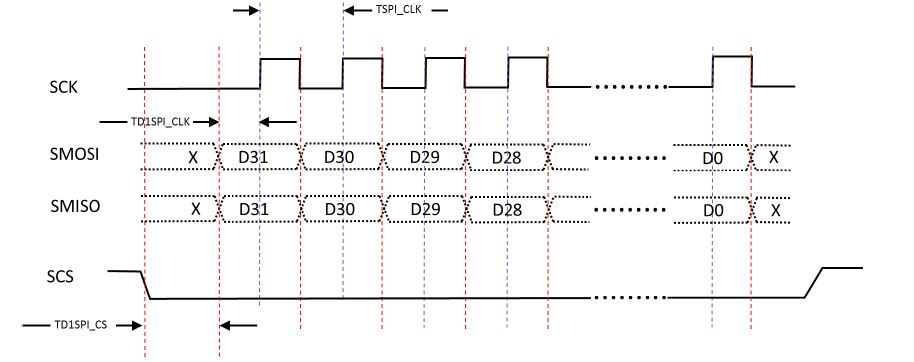
\includegraphics[width=0.9\textwidth]{SPI_Timing.jpg}
    \caption[]{SPI-Timing diagram) }
    \label{fig:SPI_Timing}
\end{figure}

The following definitions hold for the ASIC in use:


\begin{table}[H]

\caption[]{SPI Definitions}
    \label{tab:1}
    
  \begin{center}  
  \begin{tabular}{|r|l|}
  \hline
  \textbf{Name}  & \textbf{Definition} \\ \cline{1-2}
  
  \textbf{SCK} & SPI Serial Clock (output from Master) \\
  \textbf{SMOSI} &Master Output, Slave Input \\ 
  \textbf{SMISO} &Master Input, Slave Output\\
  \textbf{SCS} &Chip-Select (Active low, provided by Master)\\
  \hline
  
\end{tabular}
\end{center}
\end{table}


During one SPI communication cycle, the 32-bit word in the following configuration is sent to the ASIC serially on the SMOSI line.

\begin{table}[H]

\caption[]{Master to Slave serial bit-fields}
    \label{tab:2}
    
  \begin{center}  
  \begin{tabular}{|l|c|c|c|}
  \hline
  \textbf{Bit indices}  & 31 to 23  & 22 & 21 to 0\\ 
  \hline
  \textbf{Data Components} & SPI-Address & Read/Write Bit & SPI-Data \\
  \hline
  
\end{tabular}
\end{center}
\end{table}

The 32-bit word in the following configuration is sent from the ASIC serially on the SMISO line.

\begin{table}[H]

\caption[]{Slave to Master serial bit-fields}
    \label{tab:3}
    
  \begin{center}  
  \begin{tabular}{|l|c|c|c|}
  \hline
  \textbf{Bit indices}  & 31 to 23  & 22 & 21 to 0\\ 
  \hline
  \textbf{Data Components} & Meaningless & Meaningless & SPI-Data \\
  \hline
  
\end{tabular}
\end{center}
\end{table}
The SPI serial clock operates at minimum frequency of 1 kHz and at a maximum frequency of 5 MHz

\subsection{Design of digital hardware}
\label{sec:hardwaredesign}
\subsubsection{Introduction}

The language chosen for hardware generation is VHDL. The code was written and tested in the Libero SoC v11.7 integrated development environment. The company, which developed the environment is called Microsemi. They also provide pre-defined soft-cores such as the Core\_Uart which is used in the design. The hardware consists of a processing unit which takes commands from a computer, in the case of the CubeSat mission, this would be the on-board computer. The processing unit deciphers the input commands and interacts with the on-fabric memory as well as the ASIC. The testbenches are written in VHDL as well and the simulation software is called ModelSim and is automatically called from the Libero Interface and performs the simulation based on the specification in the testbench file. Many of the hardware components already existed in an undocumented form for the ASIC test board at PSI. The code for these components was written by Carla Brito from the company Efacec.


\subsubsection{Functional Block Diagram}

\begin{figure}[H]
    \centering
    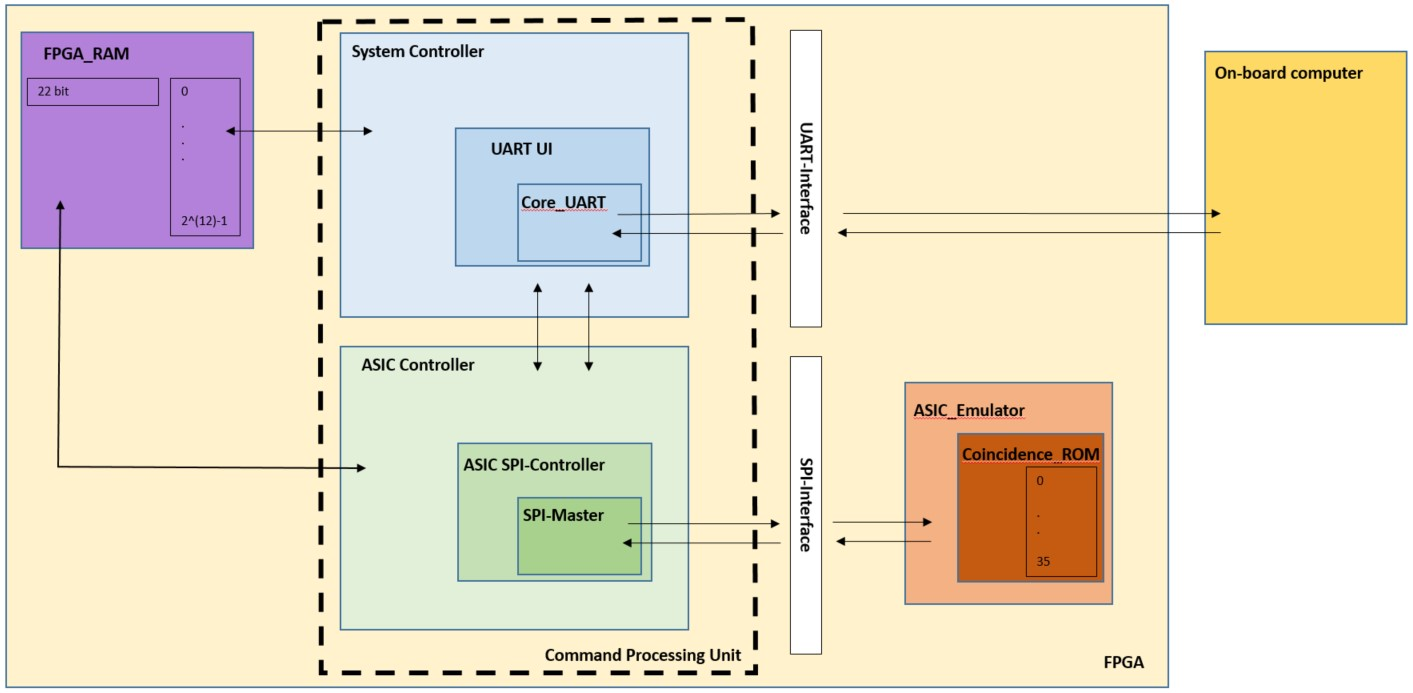
\includegraphics[width=0.9\textwidth]{Fucional_block.jpg}
    \caption[]{Functional block diagram implemented with VHDL logic) }
    \label{fig:Functional_block}
\end{figure}

The diagram above shall visualize the data flow on the FPGA architecture.

The diagram does not consider the connections and lines for the clock. In the Microsemi Libero environment, an on-board clock can be generated by connecting the output of the chip oscillator with a clock conditioning circuit, which generates the desired frequencies.
\newline

The memory on the FGPA is implemented using a RAM component. It stores data which is organized in the 22-bit format following the register size of the ASIC. It consists of 4096 readable and writeable addresses and therefore constitutes a memory of about 90 Kbit. The functionality and properties of the other blocks will be explained in their separate section later.
\newline

The oscillator in conjunction with the clock conditioning circuit generates a clock, which runs at a frequency of 20 MHz and is used for all the components except the ASIC emulator, who depends on the SPI-clock, which runs at a rate of 200 kHz.

\subsubsection{Bit-field logic of commands}
The half-duplex mode communication between the computer and the FPGA works via a serial UART interface utilizing 40-bit words.
\newline

Generally, the computer-to-FPGA commands have the following bit-field logic:

\begin{table}[H]

\caption[]{Computer-to-FPGA command constellation}
    \label{tab:4}
    
  \begin{center}  
  \begin{tabular}{|c|p{2cm}|p{2cm}|p{2.5cm}|p{2cm}|p{2cm}|}
  \hline
  \textbf{Bit indices forward}  & 39 to 36  & 35 & 34 & 33 to 22 & 21 to 0\\ 
  \hline
  \textbf{Data Components} & Command \newline Type & NO USE & Local Usage & Command Control Address & Data bits \\
  \hline
  
\end{tabular}
\end{center}
\end{table}

The FPGA-to-computer responses are in the following configuration:


\begin{table}[H]

\caption[]{FPGA-to-comuter response constellation}
    \label{tab:5}
    
  \begin{center}  
  \begin{tabular}{|c|p{3cm}|p{3cm}|p{3cm}|}
  \hline
  \textbf{Bit indices response}  & 39 to 36  & 35 to 22 & 21 to 0 \\ 
  \hline
  \textbf{Data Components} & Command Type Response & Copy of computer-to-FPGA indices for verification & Data from memory or ASIC register data or copy of computer-to-FPGA indices for verification \\
  \hline
  
\end{tabular}
\end{center}
\end{table}

To write data to an ASIC register via the SPI-port, the following sequences must be sent via the UART port:


\begin{table}[H]

\caption[]{Write ASIC register command 1/2}
    \label{tab:6}
    
  \begin{center}  
  \begin{tabular}{|c|p{2cm}|p{2cm}|p{2.5cm}|p{2cm}|p{2cm}|}
  \hline
  \textbf{Bit indices}  & 39 to 36  & 35 & 34 & 33 to 22 & 21 to 0\\ 
  \hline
  \textbf{Values} & 0001  & 0 & 0 & 0x00A & Data bits \\
  \hline
  
\end{tabular}
\end{center}
\end{table}










